% Options for packages loaded elsewhere
\PassOptionsToPackage{unicode}{hyperref}
\PassOptionsToPackage{hyphens}{url}
%
\documentclass[
  11pt,
  ignorenonframetext,
]{beamer}
\usepackage{pgfpages}
\setbeamertemplate{caption}[numbered]
\setbeamertemplate{caption label separator}{: }
\setbeamercolor{caption name}{fg=normal text.fg}
\beamertemplatenavigationsymbolsempty
% Prevent slide breaks in the middle of a paragraph
\widowpenalties 1 10000
\raggedbottom
\setbeamertemplate{part page}{
  \centering
  \begin{beamercolorbox}[sep=16pt,center]{part title}
    \usebeamerfont{part title}\insertpart\par
  \end{beamercolorbox}
}
\setbeamertemplate{section page}{
  \centering
  \begin{beamercolorbox}[sep=12pt,center]{part title}
    \usebeamerfont{section title}\insertsection\par
  \end{beamercolorbox}
}
\setbeamertemplate{subsection page}{
  \centering
  \begin{beamercolorbox}[sep=8pt,center]{part title}
    \usebeamerfont{subsection title}\insertsubsection\par
  \end{beamercolorbox}
}
\AtBeginPart{
  \frame{\partpage}
}
\AtBeginSection{
  \ifbibliography
  \else
    \frame{\sectionpage}
  \fi
}
\AtBeginSubsection{
  \frame{\subsectionpage}
}
\usepackage{lmodern}
\usepackage{amssymb,amsmath}
\usepackage{ifxetex,ifluatex}
\ifnum 0\ifxetex 1\fi\ifluatex 1\fi=0 % if pdftex
  \usepackage[T1]{fontenc}
  \usepackage[utf8]{inputenc}
  \usepackage{textcomp} % provide euro and other symbols
\else % if luatex or xetex
  \usepackage{unicode-math}
  \defaultfontfeatures{Scale=MatchLowercase}
  \defaultfontfeatures[\rmfamily]{Ligatures=TeX,Scale=1}
\fi
% Use upquote if available, for straight quotes in verbatim environments
\IfFileExists{upquote.sty}{\usepackage{upquote}}{}
\IfFileExists{microtype.sty}{% use microtype if available
  \usepackage[]{microtype}
  \UseMicrotypeSet[protrusion]{basicmath} % disable protrusion for tt fonts
}{}
\makeatletter
\@ifundefined{KOMAClassName}{% if non-KOMA class
  \IfFileExists{parskip.sty}{%
    \usepackage{parskip}
  }{% else
    \setlength{\parindent}{0pt}
    \setlength{\parskip}{6pt plus 2pt minus 1pt}}
}{% if KOMA class
  \KOMAoptions{parskip=half}}
\makeatother
\usepackage{xcolor}
\IfFileExists{xurl.sty}{\usepackage{xurl}}{} % add URL line breaks if available
\IfFileExists{bookmark.sty}{\usepackage{bookmark}}{\usepackage{hyperref}}
\hypersetup{
  pdftitle={R-programmering VT2023},
  pdfauthor={Josef Wilzén},
  hidelinks,
  pdfcreator={LaTeX via pandoc}}
\urlstyle{same} % disable monospaced font for URLs
\newif\ifbibliography
\usepackage{color}
\usepackage{fancyvrb}
\newcommand{\VerbBar}{|}
\newcommand{\VERB}{\Verb[commandchars=\\\{\}]}
\DefineVerbatimEnvironment{Highlighting}{Verbatim}{commandchars=\\\{\}}
% Add ',fontsize=\small' for more characters per line
\usepackage{framed}
\definecolor{shadecolor}{RGB}{248,248,248}
\newenvironment{Shaded}{\begin{snugshade}}{\end{snugshade}}
\newcommand{\AlertTok}[1]{\textcolor[rgb]{0.94,0.16,0.16}{#1}}
\newcommand{\AnnotationTok}[1]{\textcolor[rgb]{0.56,0.35,0.01}{\textbf{\textit{#1}}}}
\newcommand{\AttributeTok}[1]{\textcolor[rgb]{0.77,0.63,0.00}{#1}}
\newcommand{\BaseNTok}[1]{\textcolor[rgb]{0.00,0.00,0.81}{#1}}
\newcommand{\BuiltInTok}[1]{#1}
\newcommand{\CharTok}[1]{\textcolor[rgb]{0.31,0.60,0.02}{#1}}
\newcommand{\CommentTok}[1]{\textcolor[rgb]{0.56,0.35,0.01}{\textit{#1}}}
\newcommand{\CommentVarTok}[1]{\textcolor[rgb]{0.56,0.35,0.01}{\textbf{\textit{#1}}}}
\newcommand{\ConstantTok}[1]{\textcolor[rgb]{0.00,0.00,0.00}{#1}}
\newcommand{\ControlFlowTok}[1]{\textcolor[rgb]{0.13,0.29,0.53}{\textbf{#1}}}
\newcommand{\DataTypeTok}[1]{\textcolor[rgb]{0.13,0.29,0.53}{#1}}
\newcommand{\DecValTok}[1]{\textcolor[rgb]{0.00,0.00,0.81}{#1}}
\newcommand{\DocumentationTok}[1]{\textcolor[rgb]{0.56,0.35,0.01}{\textbf{\textit{#1}}}}
\newcommand{\ErrorTok}[1]{\textcolor[rgb]{0.64,0.00,0.00}{\textbf{#1}}}
\newcommand{\ExtensionTok}[1]{#1}
\newcommand{\FloatTok}[1]{\textcolor[rgb]{0.00,0.00,0.81}{#1}}
\newcommand{\FunctionTok}[1]{\textcolor[rgb]{0.00,0.00,0.00}{#1}}
\newcommand{\ImportTok}[1]{#1}
\newcommand{\InformationTok}[1]{\textcolor[rgb]{0.56,0.35,0.01}{\textbf{\textit{#1}}}}
\newcommand{\KeywordTok}[1]{\textcolor[rgb]{0.13,0.29,0.53}{\textbf{#1}}}
\newcommand{\NormalTok}[1]{#1}
\newcommand{\OperatorTok}[1]{\textcolor[rgb]{0.81,0.36,0.00}{\textbf{#1}}}
\newcommand{\OtherTok}[1]{\textcolor[rgb]{0.56,0.35,0.01}{#1}}
\newcommand{\PreprocessorTok}[1]{\textcolor[rgb]{0.56,0.35,0.01}{\textit{#1}}}
\newcommand{\RegionMarkerTok}[1]{#1}
\newcommand{\SpecialCharTok}[1]{\textcolor[rgb]{0.00,0.00,0.00}{#1}}
\newcommand{\SpecialStringTok}[1]{\textcolor[rgb]{0.31,0.60,0.02}{#1}}
\newcommand{\StringTok}[1]{\textcolor[rgb]{0.31,0.60,0.02}{#1}}
\newcommand{\VariableTok}[1]{\textcolor[rgb]{0.00,0.00,0.00}{#1}}
\newcommand{\VerbatimStringTok}[1]{\textcolor[rgb]{0.31,0.60,0.02}{#1}}
\newcommand{\WarningTok}[1]{\textcolor[rgb]{0.56,0.35,0.01}{\textbf{\textit{#1}}}}
\usepackage{longtable,booktabs}
\usepackage{caption}
% Make caption package work with longtable
\makeatletter
\def\fnum@table{\tablename~\thetable}
\makeatother
\usepackage{graphicx}
\makeatletter
\def\maxwidth{\ifdim\Gin@nat@width>\linewidth\linewidth\else\Gin@nat@width\fi}
\def\maxheight{\ifdim\Gin@nat@height>\textheight\textheight\else\Gin@nat@height\fi}
\makeatother
% Scale images if necessary, so that they will not overflow the page
% margins by default, and it is still possible to overwrite the defaults
% using explicit options in \includegraphics[width, height, ...]{}
\setkeys{Gin}{width=\maxwidth,height=\maxheight,keepaspectratio}
% Set default figure placement to htbp
\makeatletter
\def\fps@figure{htbp}
\makeatother
\setlength{\emergencystretch}{3em} % prevent overfull lines
\providecommand{\tightlist}{%
  \setlength{\itemsep}{0pt}\setlength{\parskip}{0pt}}
\setcounter{secnumdepth}{-\maxdimen} % remove section numbering
\usetheme[progressbar=frametitle,block=fill]{metropolis} %numbering=none

%%% USEFUL PACKAGES
%\usepackage{showframe} % For debugging positioning
\usepackage{etex} % If too many packages
% Encoding and language
\usepackage[utf8]{inputenc}
\usepackage{babel}
\usepackage{amsmath, amssymb}
\usepackage{natbib}
%\usepackage{booktabs}
%\usepackage{algorithmic}
\usepackage{algorithm}
\usepackage{caption}
%\usepackage{animate} % Animations
\usepackage{bm} % Bold math
\usepackage{bbm}
%\usepackage{url}
%\usepackage{pifont}
%\usepackage{ulem} % Used for strikeouts \sout
%\usepackage{stackengine}
%\usepackage{enumitem}
%\setlist[description]{leftmargin=\parindent,labelindent=\parindent}
%\usepackage{colortbl} % Used for colored rows in tables


%%% GRAPHICS
\usepackage{graphicx}
\graphicspath{{./figs/}}


%%% COLORS
\setbeamercolor{background canvas}{bg=white}
\def\BlankFrame{
	\bgroup
	%\pdfpageheight 29.7cm
	\setbeamercolor{background canvas}{bg=}
	\begin{frame}[plain]
	\end{frame}
	%\makeatletter
	%\pdfpageheight \beamer@paperheight
	%\makeatother
	\egroup}

\usepackage{xcolor}
\definecolor{DarkGreen}{HTML}{00B200}
\definecolor{LightBlue}{HTML}{0090D9}
\definecolor{gold}{rgb}{.812,.710,.231}
% Text markup
%\setbeamercolor{alerted text}{fg=red}
\newcommand{\blue}[1]{\textcolor{blue}{#1}}
\newcommand{\red}[1]{\textcolor{red}{#1}}
\newcommand{\grey}[1]{\textcolor{gray}{#1}}
\newcommand{\orange}[1]{\textcolor{mLightBrown}{#1}}
\newcommand\myheading[1]{\textbf{#1}}
\newcommand\myemph[1]{\underline{\emph{#1}}}
\newcommand\textexample[1]{\textit{\textbf{#1}}}

%%% SPACING
\newcommand\vws[1][1]{\vspace{#1\baselineskip}} % vertical white space
%\newcommand\strt[1][1.5ex]{\rule[-.05\baselineskip]{0pt}{#1}} % strut
\newcommand\strt[2]{\rule[-#1ex]{0pt}{#2ex}} % strut
\newcommand\Hrule{\vspace{1ex} \hrule \vspace{1ex}} % Horisontal rule with some space after

%%% MISC
\newcommand\articleref[4]{\noindent\begin{minipage}[t]{0.04\textwidth}
		\vspace{0pt} 
		\pgfuseimage{beamericonarticle}
	\end{minipage}%
	\begin{minipage}[t]{0.96\textwidth}
		\vspace{0pt}
		#1. \textbf{#2.} \textit{#3}, #4.
	\end{minipage}}

%%% METROPOLIS THEME SPECIFIC
\makeatletter
\setlength{\metropolis@progressonsectionpage@linewidth}{1pt}
\makeatother
%\setbeamercolor{progress bar}{fg=red,bg=red!50}


%%% TEXTPOS
\usepackage[absolute,overlay]{textpos} % option showboxes is useful in draft mode
\setlength{\TPHorizModule}{\paperwidth}
\setlength{\TPVertModule}{\paperheight}
\textblockorigin{0pt}{10mm} % start everything at top-left, below gray 


%%% TIKZ/PGFPLOTS
\usepackage{tikz}
\usetikzlibrary{arrows,positioning,calc,shapes.geometric}
%\usetikzlibrary{arrows,calc,shapes.geometric,decorations.pathmorphing,backgrounds,positioning,fit,petri,decorations.pathreplacing}
%\usepackage{pgfplots}
%\pgfplotsset{compat = 1.3}


%%% BLOCKS AND BOXES
% Changing colors of blocks
%\setbeamercolor{block title alerted}{bg=UURed,fg=palette primary.fg}
%\setbeamercolor{block body alerted}{bg=UURed!15}
\setbeamercolor{block title alerted}{bg=mLightBrown,fg=palette primary.fg}
\setbeamercolor{block body alerted}{bg=mLightBrown!15}
%\setbeamercolor{block title example}{bg=UUGreen,fg=palette primary.fg}
%\setbeamercolor{block body example}{bg=UUGreen!10}
% \mybox is a rectangular box
\usepackage{boxedminipage}
\setlength\fboxrule{2pt}
\setlength\fboxsep{2\fboxsep}
\newcommand\mybox[3][\textwidth]{
  {\color{#2}
    \begin{boxedminipage}{#1}
      {\color{palette primary.bg} #3}
    \end{boxedminipage}}%
}   
\usepackage{tcolorbox}
\tcbset{arc=1mm,grow to left by=3mm,grow to right by=3mm,left=2mm}
%\newenvironment{redbox}{%
%	\begin{tcolorbox}[colback=UURed!15,colframe=UURed]}{%
%	\end{tcolorbox}}
%\newenvironment{greenbox}{%
%	\begin{tcolorbox}[colback=UUGreen!15,colframe=UUGreen]}{%
%	\end{tcolorbox}}
\newenvironment{redbox}{%
	\begin{tcolorbox}[colback=red!15,colframe=red]}{%
	\end{tcolorbox}}
\newenvironment{greenbox}{%
	\begin{tcolorbox}[colback=DarkGreen!15,colframe=DarkGreen]}{%
	\end{tcolorbox}}
\newenvironment{graybox}{%
	\begin{tcolorbox}[colback=mDarkTeal!5,colframe=mDarkTeal]}{%
	\end{tcolorbox}}
\newenvironment{orangebox}{%
\begin{tcolorbox}[colback=mLightBrown!15,colframe=mLightBrown]}{%
	\end{tcolorbox}}
\newenvironment{bwbox}{%
	\begin{tcolorbox}[colback=white,colframe=black]}{%
\end{tcolorbox}}
\newenvironment{bluebox}{%
	\begin{tcolorbox}[colback=LightBlue!15,colframe=LightBlue]}{%
\end{tcolorbox}}


%%%%%%%%% NEW MACROS

\newcommand\imp[1]{\alert{\textbf{#1}}}
\newcommand\bfit[1]{\textbf{\textit{#1}}}
\newcommand\good{\color{DarkGreen}{$\blacktriangle$}} % used in lists
\newcommand\bad{\color{red}{$\blacktriangledown$}} % used in lists


\title{R-programmering VT2022}
\subtitle{Föreläsning 2}
\author{Josef Wilzén}
\date{2023-01-30}
\institute{Linköpings Universitet}

\begin{document}
\frame{\titlepage}

%%%%%%%%% slide %%%%%%%%%

\begin{frame}{Föreläsning 2:}
\protect\hypertarget{fuxf6reluxe4sning-2}{}


\textbf{Seminarie} på torsdag är 10:15-12:00 $\rightarrow$ se Teams!

\begin{itemize}
\tightlist
\item
  Sammanfattning: Föreläsning 1
\item
  Datastrukturer:

  \begin{itemize}
  \tightlist
  \item
    Matriser
  \item
    Data.frame
  \item
    Listor
  \end{itemize}
\item
  Databearbetning
\item
  Input och output (I/O)
\end{itemize}
\end{frame}

\hypertarget{sammanfattning-fuxf6reluxe4sning-1}{%
\section{Sammanfattning Föreläsning
1}\label{sammanfattning-fuxf6reluxe4sning-1}}

%%%%%%%%% slide %%%%%%%%%

\begin{frame}{Variabler, vektorer och typer}
\protect\hypertarget{variabler-vektorer-och-typer}{}
\begin{itemize}
\tightlist
\item
  Variabler använder vi för att spara värden

  \begin{itemize}
  \tightlist
  \item
    Sätts med \texttt{<-}
  \end{itemize}
\item
  Vektorer är en samling av likadana element

  \begin{itemize}
  \tightlist
  \item
    Skapas med \texttt{c()}
  \item
    Välj element med \texttt{[ ]}
  \end{itemize}
\item
  Beräkningar med vektorer sker elementvis och cykliskt
\item
  Värden kan vara av olika typer

  \begin{itemize}
  \tightlist
  \item
    Kollar typ med \texttt{typeof( )}
  \item
    Byter typ med \texttt{as.}
  \item
    Testa typ med \texttt{is.}
  \end{itemize}
\end{itemize}
\end{frame}

%%%%%%%%% slide %%%%%%%%%

\begin{frame}{Funktioner}
\protect\hypertarget{funktioner}{}
\begin{itemize}
\tightlist
\item
  En funktion utför något
\item
  En funktion i R är uppbyggd av

  \begin{itemize}
  \tightlist
  \item
    ett funktionsnamn, t.ex. \texttt{area}
  \item
    en funktionsdefinition: \texttt{function( )}
  \item
    0 eller flera argument, t.ex. \texttt{hojd} och \texttt{bredd}
  \item
    ``måsvingar'' \texttt{ \{ \} }
  \item
    kod, t.ex. \texttt{area <- hojd * bredd}
  \item
    returnera värde, t.ex. \texttt{return(area)}
  \end{itemize}
\end{itemize}
\end{frame}

%%%%%%%%% slide %%%%%%%%%

\begin{frame}{Logik}
\protect\hypertarget{logik}{}
\begin{itemize}
\tightlist
\item
  Logik är vanligt i programmering

  \begin{itemize}
  \tightlist
  \item
    Används i \texttt{if}-satser och indexering
  \end{itemize}
\item
  I R finns de logiska värdena \texttt{TRUE}, \texttt{FALSE}, och
  \texttt{NA}
\item
  Skapas på två olika sätt

  \begin{itemize}
  \tightlist
  \item
    Som vanliga vektorer
  \item
    Genom relationsoperatorer
  \end{itemize}
\item
  Kan användas för att välja element i vektorer
\end{itemize}
\end{frame}


\hypertarget{datastrukturer}{%
\section{Datastrukturer}\label{datastrukturer}}

%%%%%%%%% slide %%%%%%%%%

\begin{frame}{Datastrukturer}
\protect\hypertarget{datastrukturer-1}{}
\begin{itemize}
\tightlist
\item
  Lagring och hantering av data
\item
  Vi kommer att diskuttera:

  \begin{itemize}
  \tightlist
  \item
    Vektorer (Föreläsning 1)
  \item
    Matriser
  \item
    \texttt{data.frame}
  \item
    Listor
  \end{itemize}
\end{itemize}
\end{frame}

\hypertarget{matriser}{%
\section{Matriser}\label{matriser}}

%%%%%%%%% slide %%%%%%%%%

\begin{frame}{Matriser}
\protect\hypertarget{matriser-1}{}
\begin{itemize}
\tightlist
\item
  En tvådimensionell vektor
\item
  Alla element har \imp{samma} typ
\item
  Skapas med \texttt{matrix( )}
\item
  \texttt{+, -, *, /} etc. sker elementvis
\item
  Matrisoperationer finns, kommer prata mer om det senare
\item
  Hitta index med \texttt{[ "rad" , "kolumn" ]}

  \begin{itemize}
  \tightlist
  \item
    Om index för \texttt{rad} eller \texttt{kolumn} saknas väljs hela
    raden/kolumnen.
  \end{itemize}
\end{itemize}
\end{frame}

%%%%%%%%% slide %%%%%%%%%

\begin{frame}[fragile]{Matriser, exempel}
\protect\hypertarget{matriser-exempel}{}
\begin{Shaded}
\begin{Highlighting}[]
\NormalTok{en\_matris \textless{}{-}}\StringTok{ }\KeywordTok{matrix}\NormalTok{(}\DataTypeTok{data =} \DecValTok{5}\OperatorTok{:}\DecValTok{8}\NormalTok{, }\DataTypeTok{ncol =} \DecValTok{2}\NormalTok{)}
\NormalTok{en\_matris}
\end{Highlighting}
\end{Shaded}

\begin{verbatim}
##      [,1] [,2]
## [1,]    5    7
## [2,]    6    8
\end{verbatim}

\pause

\begin{Shaded}
\begin{Highlighting}[]
\NormalTok{en\_matris[}\DecValTok{1}\NormalTok{, ] \textless{}{-}}\StringTok{ }\NormalTok{en\_matris[}\DecValTok{2}\NormalTok{, ]}
\NormalTok{en\_matris}
\end{Highlighting}
\end{Shaded}

\begin{verbatim}
##      [,1] [,2]
## [1,]    6    8
## [2,]    6    8
\end{verbatim}
\end{frame}

\hypertarget{data.frame}{%
\section{data.frame}\label{data.frame}}

%%%%%%%%% slide %%%%%%%%%

\begin{frame}{data.frame}
\protect\hypertarget{data.frame-1}{}
\begin{itemize}
\tightlist
\item
  Dataset i R
\item
  Olika kolumner han ha \textcolor{red}{olika} datatyper

  \begin{itemize}
  \tightlist
  \item
    Varje kolumn är en vektor
  \end{itemize}
\item
  Indexering av variabler kan göras med variabelnamn
  \texttt{["mittNamn"]}
\item
  Kan också indexera med \texttt{[ "rad" , "kolumn" ]}
\item
  Finns många inbyggda datasets i paketet \texttt{datasets}

  \begin{itemize}
  \tightlist
  \item
    ladda in med funktionen \texttt{data( )}
  \end{itemize}
\end{itemize}
\end{frame}

%%%%%%%%% slide %%%%%%%%%

\begin{frame}[fragile]{Exempel på inbyggt dataset}
\protect\hypertarget{exempel-puxe5-inbyggt-dataset}{}
\begin{figure}
\centering
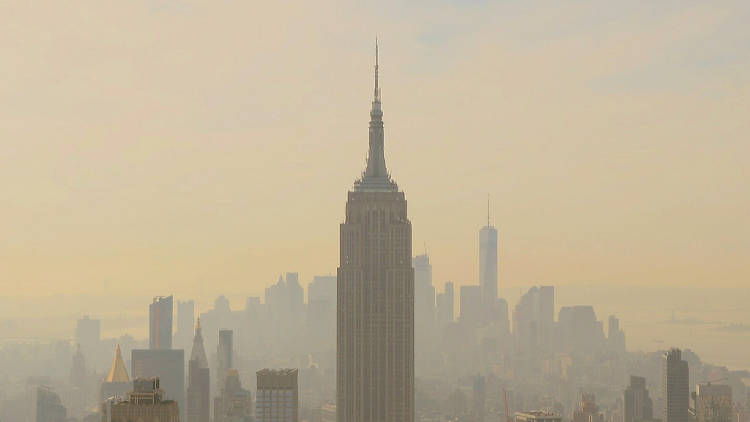
\includegraphics[width=0.5\textwidth,height=\textheight]{images/ny.jpeg}
\caption{New York}
\end{figure}

Ladda in och undersök data

\begin{Shaded}
\begin{Highlighting}[]
\KeywordTok{data}\NormalTok{(}\StringTok{"airquality"}\NormalTok{)}
\KeywordTok{head}\NormalTok{(airquality)}
\KeywordTok{tail}\NormalTok{(airquality)}
\KeywordTok{summary}\NormalTok{(airquality)}
\KeywordTok{dim}\NormalTok{(airquality)}
\end{Highlighting}
\end{Shaded}
\end{frame}

%%%%%%%%% slide %%%%%%%%%

\begin{frame}[fragile]{Skapa en data.frame}
\protect\hypertarget{skapa-en-data.frame}{}
\begin{Shaded}
\begin{Highlighting}[]
\NormalTok{minData \textless{}{-}}\StringTok{ }\KeywordTok{data.frame}\NormalTok{(}
  \DataTypeTok{namn =} \KeywordTok{c}\NormalTok{(}\StringTok{\textquotesingle{}Johan\textquotesingle{}}\NormalTok{, }\StringTok{\textquotesingle{}Therese\textquotesingle{}}\NormalTok{, }\StringTok{\textquotesingle{}Hugo\textquotesingle{}}\NormalTok{), }
  \DataTypeTok{vuxen =} \KeywordTok{c}\NormalTok{(}\OtherTok{TRUE}\NormalTok{,}\OtherTok{TRUE}\NormalTok{,}\OtherTok{FALSE}\NormalTok{), }
  \DataTypeTok{langd =} \KeywordTok{c}\NormalTok{(}\DecValTok{180}\NormalTok{,}\DecValTok{172}\NormalTok{,}\DecValTok{110}\NormalTok{))}
\NormalTok{minData}
\end{Highlighting}
\end{Shaded}

\begin{verbatim}
##      namn vuxen langd
## 1   Johan  TRUE   180
## 2 Therese  TRUE   172
## 3    Hugo FALSE   110
\end{verbatim}
\end{frame}

%%%%%%%%% slide %%%%%%%%%

\begin{frame}[fragile]{Variabler}
\protect\hypertarget{variabler}{}
\begin{itemize}
\tightlist
\item
  Varje kolumn är en vektor
\item
  Kan välja en kolumn på olika sätt, följande tar fram samma kolumn.
\end{itemize}

\begin{Shaded}
\begin{Highlighting}[]
\NormalTok{minData}\OperatorTok{$}\NormalTok{langd}
\NormalTok{minData[, }\StringTok{"langd"}\NormalTok{]}
\NormalTok{minData[[}\StringTok{"langd"}\NormalTok{]]}
\NormalTok{minData[, }\DecValTok{3}\NormalTok{]}
\NormalTok{minData[, }\KeywordTok{colnames}\NormalTok{(minData) }\OperatorTok{==}\StringTok{ "langd"}\NormalTok{]}
\end{Highlighting}
\end{Shaded}
\end{frame}

%%%%%%%%% slide %%%%%%%%%

\begin{frame}[fragile]{Nya variabler}
\protect\hypertarget{nya-variabler}{}
\begin{itemize}
\tightlist
\item
  Lägga till en ny vektor
\item
  Fungerar som vektorer
\end{itemize}

\begin{Shaded}
\begin{Highlighting}[]
\NormalTok{minData}\OperatorTok{$}\NormalTok{langdMeter \textless{}{-}}\StringTok{ }\KeywordTok{c}\NormalTok{(}\FloatTok{1.8}\NormalTok{, }\FloatTok{1.7}\NormalTok{, }\FloatTok{1.1}\NormalTok{)}
\NormalTok{minData}\OperatorTok{$}\NormalTok{rolig \textless{}{-}}\StringTok{ "Ja"}
\NormalTok{minData}
\end{Highlighting}
\end{Shaded}

\begin{verbatim}
##      namn vuxen langd langdMeter rolig
## 1   Johan  TRUE   180        1.8    Ja
## 2 Therese  TRUE   172        1.7    Ja
## 3    Hugo FALSE   110        1.1    Ja
\end{verbatim}
\end{frame}

%%%%%%%%% slide %%%%%%%%%

\begin{frame}[fragile]{Ta bort variabler}
\protect\hypertarget{ta-bort-variabler}{}
\begin{itemize}
\tightlist
\item
  Byt ut variabeln till \texttt{NULL}
\item
  Kan också plocka bort med negativ indexering
\end{itemize}

\begin{Shaded}
\begin{Highlighting}[]
\NormalTok{minData \textless{}{-}}\StringTok{ }\NormalTok{minData[, }\DecValTok{{-}4}\NormalTok{] }
\NormalTok{minData}\OperatorTok{$}\NormalTok{rolig \textless{}{-}}\StringTok{ }\OtherTok{NULL}
\NormalTok{minData}
\end{Highlighting}
\end{Shaded}

\begin{verbatim}
##      namn vuxen langd
## 1   Johan  TRUE   180
## 2 Therese  TRUE   172
## 3    Hugo FALSE   110
\end{verbatim}
\end{frame}

%%%%%%%%% slide %%%%%%%%%

\begin{frame}[fragile]{Variabelnamn}
\protect\hypertarget{variabelnamn}{}
\begin{itemize}
\tightlist
\item
  Variabelnamn är text som sparas i en vektor
\end{itemize}

\begin{Shaded}
\begin{Highlighting}[]
\KeywordTok{colnames}\NormalTok{(minData)}
\end{Highlighting}
\end{Shaded}

\begin{verbatim}
## [1] "namn"  "vuxen" "langd"
\end{verbatim}

\pause

\begin{itemize}
\tightlist
\item
  Kan byta genom att skriva över värdet
\end{itemize}

\begin{Shaded}
\begin{Highlighting}[]
\KeywordTok{colnames}\NormalTok{(minData)[}\DecValTok{2}\NormalTok{] \textless{}{-}}\StringTok{ "Inte Barn"}
\NormalTok{minData}
\end{Highlighting}
\end{Shaded}

\begin{verbatim}
##      namn Inte Barn langd
## 1   Johan      TRUE   180
## 2 Therese      TRUE   172
## 3    Hugo     FALSE   110
\end{verbatim}
\end{frame}

%%%%%%%%% slide %%%%%%%%%

\begin{frame}[fragile]{Rader}
\protect\hypertarget{rader}{}
\begin{itemize}
\tightlist
\item
  Varje rad har sitt egna ID
\item
  Alla rad IDn är en textvektor
\end{itemize}

\begin{Shaded}
\begin{Highlighting}[]
\KeywordTok{rownames}\NormalTok{(minData)}
\end{Highlighting}
\end{Shaded}

\begin{verbatim}
## [1] "1" "2" "3"
\end{verbatim}

\pause

\begin{itemize}
\tightlist
\item
  Kan byta precis som med variabler
\end{itemize}

\begin{Shaded}
\begin{Highlighting}[]
\KeywordTok{rownames}\NormalTok{(minData)[}\DecValTok{1}\NormalTok{] \textless{}{-}}\StringTok{ "Person 1"}
\NormalTok{minData}
\end{Highlighting}
\end{Shaded}

\begin{verbatim}
##             namn Inte Barn langd
## Person 1   Johan      TRUE   180
## 2        Therese      TRUE   172
## 3           Hugo     FALSE   110
\end{verbatim}
\end{frame}

\hypertarget{listor}{%
\section{Listor}\label{listor}}

%%%%%%%%% slide %%%%%%%%%

\begin{frame}[fragile]{Listor}
\protect\hypertarget{listor-1}{}
\begin{itemize}
\tightlist
\item
  En lista är en samling objekt
\item
  Tänk en vektor där varje element är en låda

  \begin{itemize}
  \tightlist
  \item
    Lådan kan innehålla ``vad som helst''
  \end{itemize}
\end{itemize}

\begin{Shaded}
\begin{Highlighting}[]
\NormalTok{minLista \textless{}{-}}\StringTok{ }\KeywordTok{list}\NormalTok{(}\DataTypeTok{namn =} \StringTok{"Ash Ketchum"}\NormalTok{,}
             \KeywordTok{c}\NormalTok{(}\StringTok{"Pikachu"}\NormalTok{, }\StringTok{"Caterpie"}\NormalTok{, }\StringTok{"Charmander"}\NormalTok{))}
\NormalTok{minLista}
\end{Highlighting}
\end{Shaded}

\begin{verbatim}
## $namn
## [1] "Ash Ketchum"
## 
## [[2]]
## [1] "Pikachu"    "Caterpie"   "Charmander"
\end{verbatim}
\end{frame}

%%%%%%%%% slide %%%%%%%%%

\begin{frame}[fragile]{Indexering i listor}
\protect\hypertarget{indexering-i-listor}{}
\begin{itemize}
\tightlist
\item
  Indexering görs med hakparanteser

  \begin{itemize}
  \tightlist
  \item
    För att komma åt ett eller flera objekt: \texttt{[ ]}
  \item
    För att komma åt innehållet i ett objekt: \texttt{[[ ]]}
  \end{itemize}
\item
  Om namngivna objekt:

  \begin{itemize}
  \tightlist
  \item
    \textbackslash texttt\{minLista\$namn\}
  \item
    \texttt{minList[["namn"]]}
  \end{itemize}
\end{itemize}

\begin{Shaded}
\begin{Highlighting}[]
\NormalTok{minLista[}\DecValTok{1}\NormalTok{]}
\end{Highlighting}
\end{Shaded}

\begin{verbatim}
## $namn
## [1] "Ash Ketchum"
\end{verbatim}

\begin{Shaded}
\begin{Highlighting}[]
\NormalTok{minLista[[}\DecValTok{1}\NormalTok{]]}
\end{Highlighting}
\end{Shaded}

\begin{verbatim}
## [1] "Ash Ketchum"
\end{verbatim}
\end{frame}

\hypertarget{databearbetning}{%
\section{Databearbetning}\label{databearbetning}}

%%%%%%%%% slide %%%%%%%%%

\begin{frame}{Sammanfoga data}
\protect\hypertarget{sammanfoga-data}{}
\begin{itemize}
\tightlist
\item
  Man vill ofta kombinera olika dataset
\item
  Vanliga sammanslagningar

  \begin{itemize}
  \tightlist
  \item
    Kombinera rader \texttt{rbind( )}
  \item
    Kombinera kolumner \texttt{cbind( )}
  \item
    Kombinera datasets \texttt{merge( )}
  \end{itemize}
\item
  Om man vill aggregera data används \texttt{aggregate( )}
\end{itemize}
\end{frame}

\hypertarget{input-och-output}{%
\section{Input och Output}\label{input-och-output}}

%%%%%%%%% slide %%%%%%%%%

\begin{frame}{Input}
\protect\hypertarget{input}{}
\begin{itemize}
\tightlist
\item
  Att läsa in data

  \begin{itemize}
  \tightlist
  \item
    Från filer på datorn/nätverket
    (\texttt{.csv .xlsx .txt .Rdata .RDS})
  \item
    Filer från webben (\texttt{httr})
  \item
    Från databaser (\texttt{SQL})
  \item
    Via något API (\texttt{rOpenGov})
  \end{itemize}
\end{itemize}

\pause

\begin{itemize}
\tightlist
\item
  För att läsa in filer i R använder vi

  \begin{itemize}
  \tightlist
  \item
    \texttt{.csv} och \texttt{.txt}

    \begin{itemize}
    \tightlist
    \item
      \texttt{read.table( )}, \texttt{read.csv( )} och
      \texttt{read.csv2( )}
    \end{itemize}
  \item
    \texttt{.Rdata}

    \begin{itemize}
    \tightlist
    \item
      \texttt{load( )}
    \end{itemize}
  \item
    \texttt{.RDS}

    \begin{itemize}
    \tightlist
    \item
      \texttt{readRDS( )}
    \end{itemize}
  \end{itemize}
\end{itemize}
\end{frame}

%%%%%%%%% slide %%%%%%%%%

\begin{frame}{Output}
\protect\hypertarget{output}{}
\begin{itemize}
\tightlist
\item
  Att leverera data

  \begin{itemize}
  \tightlist
  \item
    Filer
  \item
    Databaser/API
  \item
    Interaktiva webbdatabaser (\texttt{Shiny})
  \item
    Rapporter/analyser/texter (\texttt{knitr})

    \begin{itemize}
    \tightlist
    \item
      Detta kommer i miniprojekten
    \end{itemize}
  \end{itemize}
\end{itemize}

\pause

\begin{itemize}
\tightlist
\item
  För att spara filer i R använder vi

  \begin{itemize}
  \tightlist
  \item
    \texttt{.csv}

    \begin{itemize}
    \tightlist
    \item
      \texttt{write.table( )}, \texttt{write.csv( )} och
      \texttt{write.csv2( )}
    \end{itemize}
  \item
    \texttt{.Rdata}

    \begin{itemize}
    \tightlist
    \item
      \texttt{save( )}
    \end{itemize}
  \item
    \texttt{.RDS}

    \begin{itemize}
    \tightlist
    \item
      \texttt{saveRDS( )}
    \end{itemize}
  \end{itemize}
\end{itemize}
\end{frame}

\end{document}
